\documentclass[11pt,a4paper]{article}
\usepackage[margin=2.5cm]{geometry}
\usepackage{amsmath}
\usepackage{graphicx}

\title{Labwork 3: Hello, CUDA!}
\author{Duong Tan Binh \\ Student ID: 2540007}
\date{}

\begin{document}
\maketitle

\section{Method}
I read \texttt{input.jpg} with \texttt{imread}. The image is 512 pixels wide
and 600 pixels high. I reshape it to \texttt{(512 * 600, 3)} and calculate
the gray value of each pixel:
\[
\text{gray} = (R + G + B) / 3
\]
On the CPU, I use a \texttt{for} loop. On the GPU, each thread handles one
pixel. Its index is \texttt{threadIdx.x + blockIdx.x * blockDim.x}.
I check that the index is smaller than the number of pixels.
I convert R, G and B to integers before adding them to avoid overflow.

\section{Results}
I use \texttt{time.time()} to measure the CPU and GPU times.
I run the kernel once before timing so compilation is not included.
I then measure each block size once. GPU time includes copying the image
to the GPU and copying the result back. I divide CPU time by GPU time
to get the speedup.

\begin{verbatim}
CPU time: 120.655 ms
Block size: 32
GPU time: 0.52 ms
Speedup: 232.25
Block size: 64
GPU time: 0.541 ms
Speedup: 223.03
Block size: 128
GPU time: 0.356 ms
Speedup: 338.5
Block size: 256
GPU time: 0.348 ms
Speedup: 346.38
Block size: 512
GPU time: 0.331 ms
Speedup: 364.34
Block size: 1024
GPU time: 0.331 ms
Speedup: 364.34
\end{verbatim}

\newpage
\section{Comments}
The CPU and GPU give the same grayscale image.
The CPU takes 120.655 ms. Block sizes 512 and 1024 both take about
0.331 ms, giving a speedup of about 364.
A larger block is not always faster: block size 64 takes slightly longer
than 32. I only measured each size once, so these small differences may
change in another run.

\begin{center}
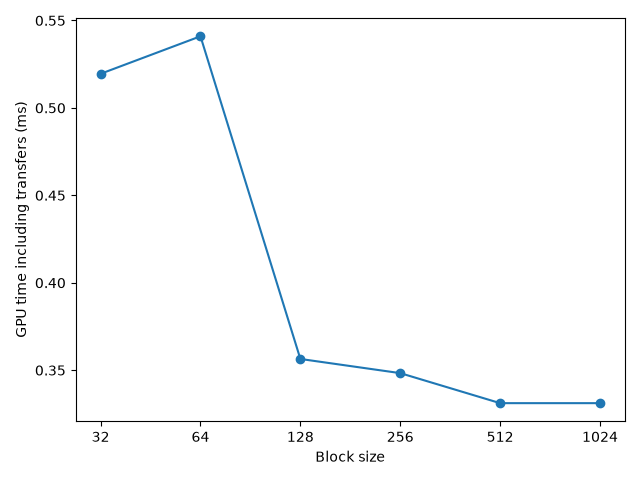
\includegraphics[width=0.85\textwidth]{block_size_time.png}
\end{center}

\begin{center}
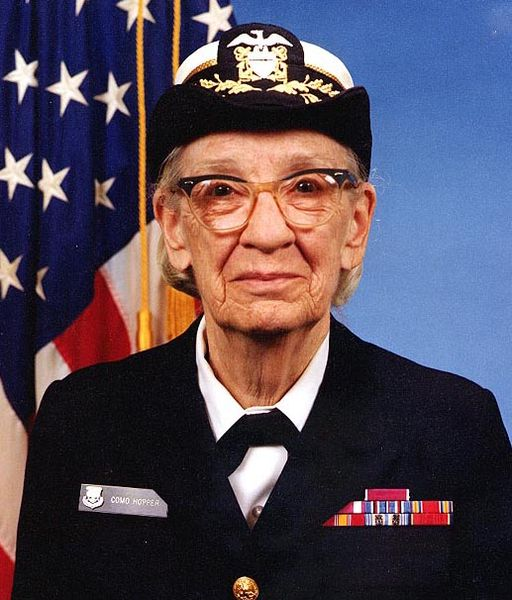
\includegraphics[width=0.30\textwidth]{input.jpg}
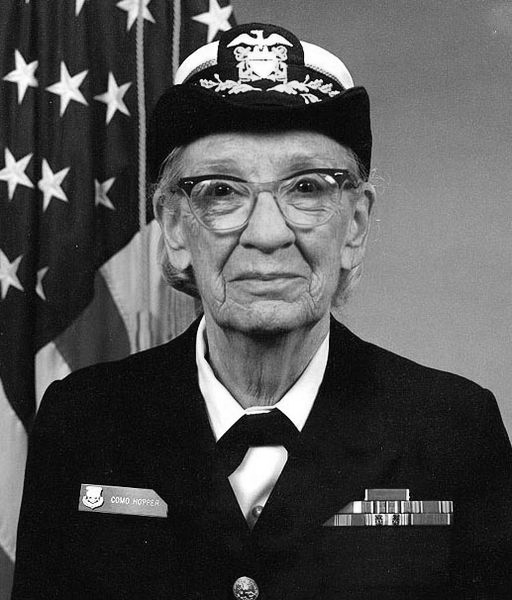
\includegraphics[width=0.30\textwidth]{gray_cpu.png}
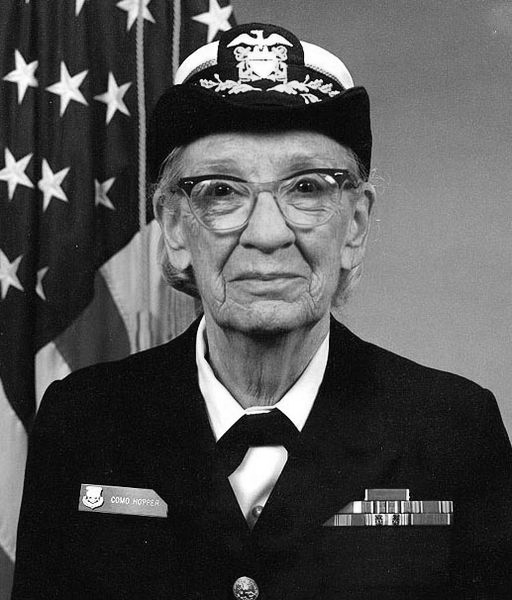
\includegraphics[width=0.30\textwidth]{gray_gpu.png}
\end{center}
From left to right: input image, CPU result, GPU result.

\end{document}
